\section{LEVEL 6 · Kansen berekenen}

\begin{missie}
Missie: bereken hoe waarschijnlijk iets is met de normale verdeling. (LPD 14)
\end{missie}

\begin{doel}
\textbf{DOEL} \quad Na dit level kan je:

☐ een kans bij een normale verdeling voorstellen als een \textbf{oppervlakte} onder de Gausskromme;

☐ kansen berekenen van de vorm $P(X<a)$, $P(X>a)$ en $P(a<X<b)$ met \textbf{ICT};

☐ een antwoord correct \textbf{interpreteren} met een antwoordzin en nagaan of het realistisch is;

☐ uit een kans het \textbf{verwacht aantal} personen berekenen.
\end{doel}

\subsection*{Theorie 6.1 · Kans = oppervlakte}

\begin{theorie}
Bij een normaal verdeelde variabele $X\sim N(\mu,\sigma)$ is de \textbf{kans} dat $X$ in een interval ligt gelijk aan de \textbf{oppervlakte} onder de Gausskromme boven dat interval. De totale oppervlakte is 1 (= 100 \%), dus elke kans ligt tussen 0 en 1.

\begin{itemize}
\item $P(X\le a)$: de oppervlakte links van $a$.
\item $P(X\ge a)=1-P(X\le a)$: de oppervlakte rechts van $a$.
\item $P(a\le X\le b)=P(X\le b)-P(X\le a)$: de oppervlakte tussen $a$ en $b$.
\item Bij een continue variabele is $P(X=a)=0$. Daarom maakt het niet uit of je < of ≤ schrijft.
\item Door de symmetrie is $P(X<\mu)=0{,}5$ en $P(X<\mu-c)=P(X>\mu+c)$.
\end{itemize}
\end{theorie}

\begin{center}
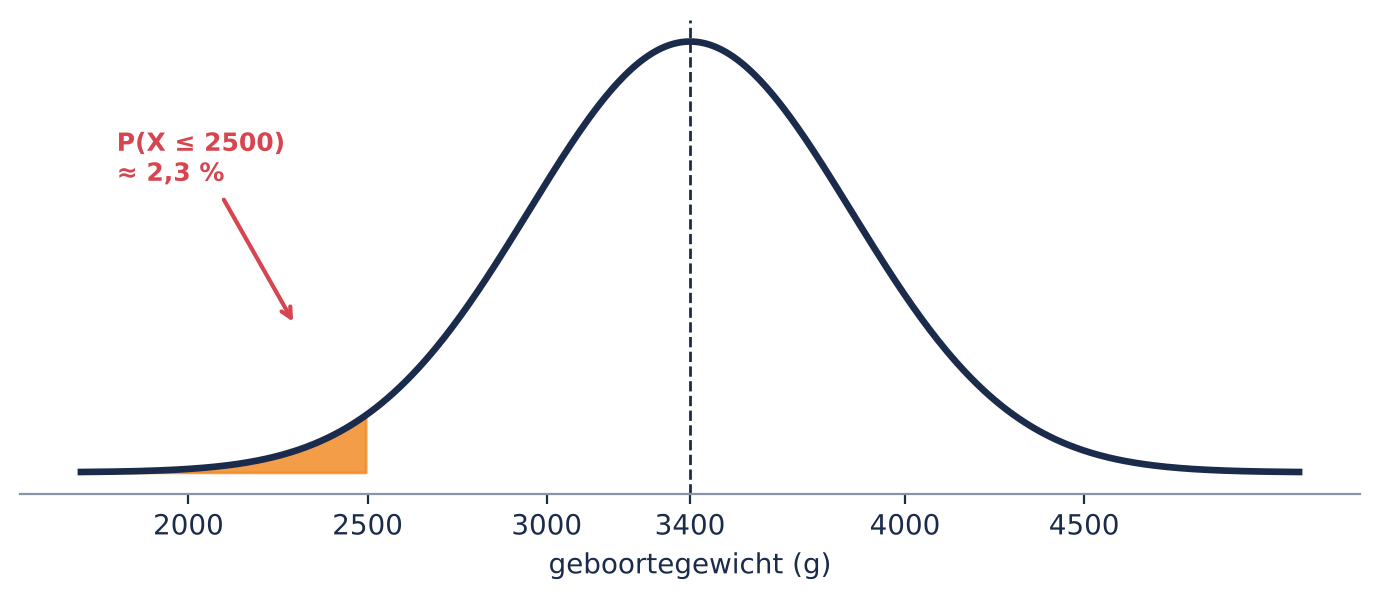
\includegraphics[width=0.8\textwidth]{figuren/l6_geboortegewicht.png}
\end{center}

\begin{ict}
\textbf{ICT-TIP: kansen berekenen.} Je zoekt telkens $P(X\le a)$ of $P(a\le X\le b)$.

• \emph{Rekentoestel (TI):} 2nd VARS $\rightarrow$ normalcdf(ondergrens, bovengrens, $\mu$, $\sigma$). Voor ‘links’ of ‘rechts’ gebruik je een heel grote grens: $-10^{99}$ of $10^{99}$ (op de TI: $-$1E99 en 1E99). Op Casio: DISTR $\rightarrow$ NORM $\rightarrow$ Ncd.

• \emph{GeoGebra:} Normaal($\mu$, $\sigma$, $a$, Waar) geeft $P(X\le a)$. Of gebruik het venster Kansrekening.

• \emph{Excel:} =NORM.VERD($a$; $\mu$; $\sigma$; WAAR) geeft $P(X\le a)$.

Menu’s en namen verschillen per toestel of versie: zoek ‘normale verdeling’ of ‘normal cdf’.
\end{ict}

\begin{theorie}
\textbf{Stappenplan voor een kansvraag}

\begin{enumerate}
\item \textbf{Noteer} de variabele en het model: $X\sim N(\mu,\sigma)$.
\item \textbf{Schets} de Gausskromme en arceer de gevraagde oppervlakte.
\item \textbf{Bereken} de kans met ICT.
\item \textbf{Antwoordzin}: zeg wat de kans betekent in de context en controleer of het antwoord realistisch is.
\end{enumerate}
\end{theorie}

\begin{voorbeeld}
\textbf{Voorbeeld.} Het geboortegewicht van baby’s is normaal verdeeld met $\mu=3400$ g en $\sigma=450$ g. Een baby met een gewicht onder 2500 g heeft een ‘laag geboortegewicht’. Wat is de kans dat een baby een laag geboortegewicht heeft?

\textbf{1.} $X$ = geboortegewicht (g), $X\sim N(3400;\,450)$.

\textbf{2.} Schets: de oppervlakte links van 2500 (zie de grafiek).

\textbf{3.} $P(X<2500)=\text{normalcdf}(-10^{99};\,2500;\,3400;\,450)\approx 0{,}0228$.

\textbf{4.} Antwoordzin: de kans op een laag geboortegewicht is ongeveer 2,3 \%; dus ongeveer 2 à 3 op 100 baby’s. Dat is realistisch: 2500 g ligt $2\sigma$ onder het gemiddelde en de 68 – 95 – 99,7-regel geeft ongeveer 2,5 \%.

\textbf{Meer vragen:} $P(X>4000)\approx 0{,}0912$ \quad en \quad $P(3000<X<3800)\approx 0{,}6259$.
\end{voorbeeld}

\begin{letop}
\textbf{LET OP} \quad Een kans is een getal tussen 0 en 1 (of tussen 0 \% en 100 \%). Krijg je 1,2 of $-0{,}3$? Dan heb je een fout gemaakt. Controleer ook met de schets: een klein gearceerd gebied moet een kleine kans geven.
\end{letop}

\subsection*{Aan de slag}

\subsubsection*{Oefening 6.1 \quad ★☆☆ \quad Stap voor stap}

Gebruik de baby’s uit het voorbeeld: $X\sim N(3400;\,450)$. Bereken $P(X<3000)$.

\textbf{1.} Noteer het model. \lijn

\textbf{2.} Schets de kromme en arceer de gevraagde oppervlakte (links van 3000). \lijn

\textbf{3.} Bereken met ICT. \lijn

\textbf{4.} Antwoordzin. \lijn

\begin{oplossing}
\textbf{Oplossing 6.1}

$P(X<3000)=\text{normalcdf}(-10^{99};\,3000;\,3400;\,450)\approx 0{,}1870$. Antwoordzin: de kans dat een baby minder dan 3000 g weegt, is ongeveer 18,7 \%. Realistisch: 3000 g ligt minder dan $1\sigma$ onder het gemiddelde, dus de kans is kleiner dan 50 \% maar groter dan 16 \%.
\end{oplossing}

\subsubsection*{Oefening 6.2 \quad ★★☆ \quad Koppel: schets en notatie}

Verbind elke figuur met de juiste kans (de oranje oppervlakte is gevraagd).

\begin{center}
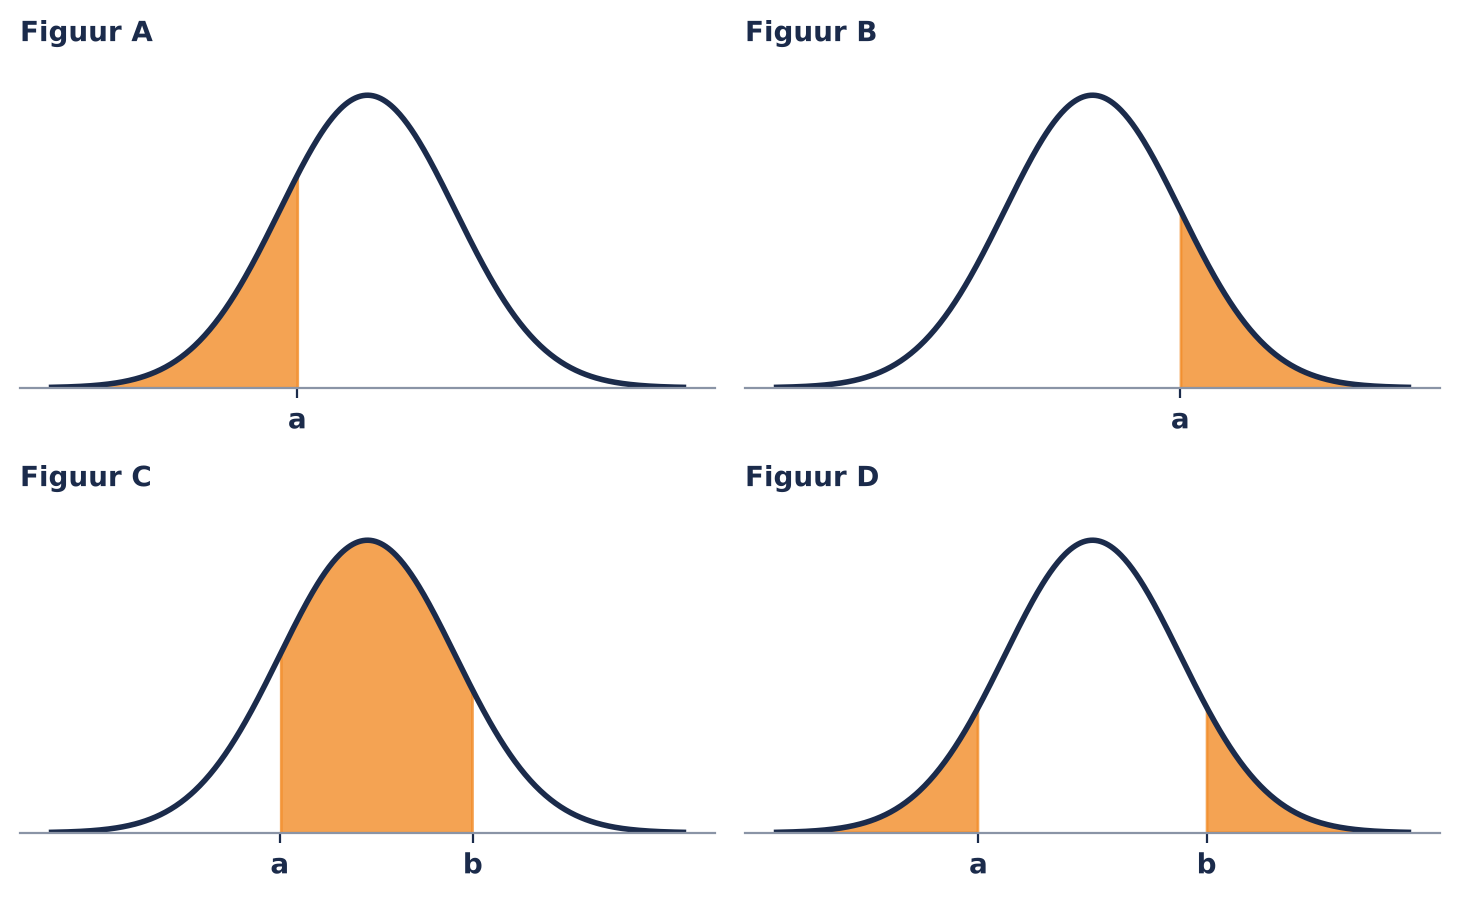
\includegraphics[width=0.85\textwidth]{figuren/l6_gearceerd.png}
\end{center}

1. $P(X<a)$ \qquad 2. $P(X>a)$ \qquad 3. $P(a<X<b)$ \qquad 4. $P(X<a)+P(X>b)$

Figuur A: \_\_\_ \qquad Figuur B: \_\_\_ \qquad Figuur C: \_\_\_ \qquad Figuur D: \_\_\_

\begin{oplossing}
\textbf{Oplossing 6.2}

A – 1 \quad B – 2 \quad C – 3 \quad D – 4
\end{oplossing}

\subsubsection*{Oefening 6.3 \quad ★★☆ \quad Context: slaapduur}

De slaapduur (in uur) van leerlingen van de derde graad is normaal verdeeld met $\mu=7{,}5$ en $\sigma=1{,}1$. Bereken met ICT de kans dat een leerling:

\textbf{a)} minder dan 6 uur slaapt; \quad \textbf{b)} meer dan 9 uur slaapt; \quad \textbf{c)} tussen 7 en 8,5 uur slaapt. \lijn

\textbf{d)} Wat valt je op bij a) en b)? Verklaar met de symmetrie van de kromme. \lijn

\textbf{e)} In een school zitten 400 leerlingen van de derde graad. Hoeveel verwacht je er die tussen 7 en 8,5 uur slapen? \lijn

\begin{oplossing}
\textbf{Oplossing 6.3}

a) $P(X<6)\approx 0{,}0863$. b) $P(X>9)\approx 0{,}0863$. c) $P(7<X<8{,}5)\approx 0{,}4936$. d) De kansen zijn gelijk: 6 en 9 liggen even ver van $\mu=7{,}5$ (telkens 1,5 uur), en de kromme is symmetrisch. e) $400\cdot 0{,}4936\approx 197$ leerlingen (ongeveer 197 op 400, bijna de helft).
\end{oplossing}

\subsubsection*{Oefening 6.4 \quad ★★☆ \quad Context: fietshelmen}

Een kinderopvang bestelt fietshelmen voor 6-jarigen. De hoofdomtrek is normaal verdeeld met $\mu=52$ cm en $\sigma=1{,}5$ cm. De bestelde helm past bij een hoofdomtrek tussen 50 en 54 cm.

\textbf{a)} Wat is de kans dat de helm een kind past? Antwoordzin. \lijn

\textbf{b)} De opvang heeft 60 kinderen van 6 jaar. Voor hoeveel kinderen verwacht je dat de helm past? \lijn

\textbf{c)} Wat is de kans dat een kind een kleinere helm nodig heeft (omtrek kleiner dan 50 cm)? \lijn

\begin{oplossing}
\textbf{Oplossing 6.4}

a) $P(50<X<54)\approx 0{,}8176$. De helm past bij ongeveer 81,8 \% van de kinderen. b) $60\cdot 0{,}8176\approx 49$ kinderen. c) $P(X<50)\approx 0{,}0912$: ongeveer 9,1 \%.
\end{oplossing}

\subsubsection*{Oefening 6.5 \quad ★★☆ \quad De regel controleren}

Neem opnieuw $X\sim N(3400;\,450)$.

\textbf{a)} Bereken $P(\mu-\sigma<X<\mu+\sigma)$, $P(\mu-2\sigma<X<\mu+2\sigma)$ en $P(\mu-3\sigma<X<\mu+3\sigma)$. \lijn

\textbf{b)} Vergelijk met de 68 – 95 – 99,7-regel. Wat besluit je? \lijn

\begin{oplossing}
\textbf{Oplossing 6.5}

a) $P(2950<X<3850)\approx 0{,}6827$; $P(2500<X<4300)\approx 0{,}9545$; $P(2050<X<4750)\approx 0{,}9973$. b) Dezelfde resultaten als de regel, maar nauwkeuriger; de regel is dus een handige benadering.
\end{oplossing}

\subsubsection*{Oefening 6.6 \quad ★★★ \quad Probleemoplossend: een planning maken}

Een bezoek van een thuisverpleegkundige duurt gemiddeld 35 minuten met een standaardafwijking van 6 minuten (normale verdeling). Ze plant voor elk bezoek 40 minuten.

\textbf{a)} Wat is gegeven en wat wordt gevraagd? Noteer het model. \lijn

\textbf{b)} Wat is de kans dat een bezoek uitloopt (langer duurt dan 40 minuten)? \lijn

\textbf{c)} Ze doet 25 bezoeken per week. Hoeveel bezoeken zullen naar verwachting uitlopen? \lijn

\textbf{d)} Is het redelijk dat ze 40 minuten plant? Beargumenteer in twee zinnen. \lijn

\begin{oplossing}
\textbf{Oplossing 6.6}

a) Gegeven: $\mu=35$ min, $\sigma=6$ min; gevraagd: de kans dat $X>40$. Model: $X\sim N(35;\,6)$. b) $P(X>40)\approx 0{,}2023$ (ongeveer 20 \%). c) $25\cdot 0{,}2023\approx 5$ bezoeken. d) Eén bezoek op vijf loopt uit; dat is niet weinig. Als ze meer zekerheid wil, plant ze beter meer tijd in (bv. 45 minuten); de kans op uitlopen daalt dan sterk (ongeveer 5 \%).
\end{oplossing}

\subsubsection*{Oefening 6.7 \quad ★★★ \quad Extra: z-score en vergelijken (niet in de toets)}

De \textbf{z-score} $z=\dfrac{x-\mu}{\sigma}$ geeft aan hoeveel standaardafwijkingen een waarde van het gemiddelde ligt. Jana haalde 70 op een toets met $\mu=60$ en $\sigma=8$. Bram haalde 62 op een andere toets met $\mu=50$ en $\sigma=6$.

\textbf{a)} Bereken de z-scores van beide leerlingen. \lijn

\textbf{b)} Wie presteerde, ten opzichte van de eigen groep, het best? \lijn

\begin{oplossing}
\textbf{Oplossing 6.7}

a) $z_{\text{Jana}}=\dfrac{70-60}{8}=1{,}25$; $z_{\text{Bram}}=\dfrac{62-50}{6}=2$. b) Bram: hij ligt 2 standaardafwijkingen boven het gemiddelde van zijn groep, Jana slechts 1,25.
\end{oplossing}

\subsection*{Invullen · kansen en oppervlakte}

\textbf{Woordenlijst:} oppervlakte – 1 – symmetrie – ICT – antwoordzin – 0.

Bij een normale verdeling is een kans gelijk aan een \gat{oppervlakte} onder de Gausskromme. De totale oppervlakte is \gat{1}. Met \gat{ICT} bereken je de kans. Om te controleren of je antwoord realistisch is, maak je een schets en schrijf je een \gat{antwoordzin}. Door \gat{symmetrie} is $P(X<\mu-c)=P(X>\mu+c)$. Bij een continue variabele is de kans $P(X=a)$ gelijk aan \gat{0}.

\subsection*{Foutjager}

\textbf{1.} Lars: ‘$P(X>5)=1{,}3$.’ \lijn

\textbf{2.} Eva: ‘Omdat $P(X=170)=0$, kan niemand 170 cm groot zijn.’ \lijn

\textbf{3.} Sam: ‘$P(a<X<b)=P(X\le a)-P(X\le b)$.’ \lijn

\begin{oplossing}
\textbf{Oplossing Foutjager}

1. Een kans is nooit groter dan 1. 2. $P(X=170)=0$ is de kans op exact 170,0000… cm; dat is bij een continue variabele altijd 0, maar mensen met ongeveer 170 cm bestaan wel (kans op een interval is positief). 3. Het moet $P(X\le b)-P(X\le a)$ zijn; anders krijg je een negatieve kans.
\end{oplossing}

\subsection*{CHECK · Level 6}

Het gewicht van pakjes babymelk is normaal verdeeld met $\mu=500$ g en $\sigma=4$ g.

\textbf{1.} (2 p) Bereken $P(X<495)$ en schrijf een antwoordzin. \lijn

\textbf{2.} (2 p) Bereken $P(496<X<504)$. Welke regel kan je gebruiken om te controleren? \lijn

\textbf{3.} (2 p) Een fabriek maakt 10\,000 pakjes. Hoeveel verwacht je er die lichter zijn dan 492 g? \lijn

\begin{doel}
\textbf{Score:} \_\_\_ / 6 \quad ☐ behaald (vanaf 4 / 6) \quad ☐ nog even oefenen
\end{doel}

\begin{oplossing}
\textbf{Oplossing CHECK 6}

1. $P(X<495)\approx 0{,}1056$: ongeveer 10,6 \% van de pakjes is lichter dan 495 g. 2. $P(496<X<504)=P(\mu-\sigma<X<\mu+\sigma)\approx 0{,}6827$; controle met de 68-regel. 3. 492 g is $\mu-2\sigma$; $P(X<492)\approx 0{,}0228$, dus ongeveer $10\,000\cdot 0{,}0228\approx 228$ pakjes.
\end{oplossing}
